\documentclass[12pt]{report}
\usepackage{style}
\usepackage{mathtools}
\author{Aaron Power}
\begin{document}
\chapter{CA1 Usability}
\section{Analysis}
The research question posed is "Is there a significant difference in the mean time taken to find 3 star hotel list between two websites, \textit{discoverireland.ie}, and \textit{discovernorthernireland.com}?". The usability researchers have decided to set their risk of a flase positive decision (\textit{a}) to 5\%.

For the collection of data students, were grouped into pairs, and recorded the time take to display the list of 3 star hotels for each location. A toss of a coin was used to determine which site was searched first. Since, a single parcipant parpicpanted in both tests, a paired t-test is the most suitable experimental design for the study.

\section{Data}
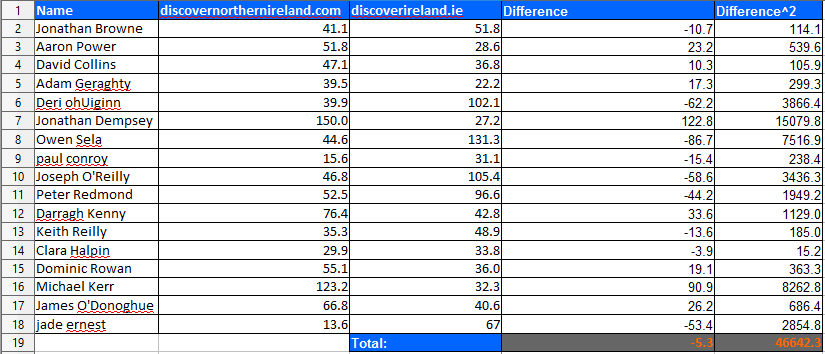
\includegraphics{exceltable.png}
\section{Formulas}
\begin{align*}
     d &= \text{number of participants.} \\
     \overline{d} &= \text{average difference.} \\
     S^2_d &= \frac{\sum d_{i^2} - \frac{(\sum d_i)^2}{d}}{d-1} \\
     t &= \frac{\overline{d} - 0}{\frac{sd}{\sqrt{d}}} \\
\end{align*}

\section{Solution}
\subsection{Hypothesis}
The null hypothesis can be expressed formally as:
\[ H_o: u_1 - u_2 = 0 \text{ or } u_1 = u_2 \text{ for all 17 observations.}\]
The alternative hypothesis is
\[H_1: u_1 \neq u_2\]

\subsection{Calculate the test statistic}

\[t = \frac{\overline{d} - 0}{\frac{S_d}{\sqrt{d}}}\]
with \(d - 1\) degrees of freedom

\begin{align*}
d &= 17\\
\overline{d} &= \frac{-5.3}{17} = 0.3117\\
S^2_d &= \frac{46642.3 - \frac{-5.3^2}{17}}{16}\\
S_d &= \sqrt{\frac{46642.3 - \frac{-5.3^2}{17}}{16}}
= \sqrt{\frac{46642.3 - 1.6523}{16}}
= \sqrt{\frac{46640.6476}{16}}
= \sqrt{2915.0404}
= 53.9911\\
t &= \frac{0.3117}{\frac{53.9911}{\sqrt{17}}}
= \frac{0.3117}{4.1231}
= 0.07559\\
\end{align*}


\subsection{Make the decision}
The \textbf{t} with 16 degrees of freedom and having cumulative probabilities of 97.5\% (as the test is two-tailed with \(a\) = 0.05) the critical values of \(\pm2.120\) are obtained.  As the calculated \textbf{t} is 0.07559 falls well outside the critical region(s) we fail to reject the hypothesis of no difference in load times of the websites. It is important to note that as the sample size is reasonably small, the type 2 error (or false negative) rate could be high.  This can be reduced by conducting a larger study.
larger study. 
\end{document}
